% !TEX root = ../main.tex
Результати теорем \ref{main_th} та \ref{cond_th} можуть бути застосовані
з теоремою про неперервне відображення \ref{th:cont_map}. % з \cite{Resnick_2007}. 
% В термінах грубої збіжності точкових процесів, її можна сформулювати наступним чином:
% \begin{theorem}[теорема про неперервне відображення]\label{cmt}
%     Нехай $\varphi$ є неперервним відображенням з простору
%     $\mathcal{M}^p_{[0,1]}$ точкових мір на $[0,1]$
%     з грубою топологією в $\R$ зі стандартною топологією.
%     Якщо $\xi_n$ --- послідовність точкових процесів,
%     що грубо збігається за розподілом до $\xi$, $\xi_n \overset{vd}{\longrightarrow} \xi$,
%     тоді 
%     $\varphi(\xi_n) \overset{d}{\longrightarrow} \varphi(\xi)$,
%     тобто послідовність випадкових величин $\varphi(\xi_n)$ збігається за розподілом
%     до $\varphi(\xi)$.
% \end{theorem}
% \begin{remark}
%     За означенням збіжності за розподілом, якщо $\varphi$ є обмеженою, то також
%     має місце
%     $\E\varphi(\xi_n) \to \E\varphi(\xi)$.
% \end{remark}
% Перед дослідженням граничних розподілів для деяких відображень,
% варто навести твердження 3.13 з \cite{Resnick_1987},
% яке можна сформулювати наступним чином:
% \begin{lemma}\label{point_conv}
%     Нехай $\mu_n$ --- грубо збіжна послідовність точкових мір в $\mathcal{M}^p_{[0,1]}$, тобто $\mu_n \overset{v}{\longrightarrow} \mu$.
%     Тоді
%     \begin{equation*}
%         \mu_n = \sum_{i=1}^k \delta_{x_i^{(n)}}, \;
%         \mu = \sum_{i=1}^k \delta_{x_i}
%     \end{equation*} 
%     де $\delta_x$ є мірою Дірака, зосередженою в $x$,
%     а $x_i^{(n)} \to x_i, n\to\infty$ для $i=1,\dots,k$.
% \end{lemma}
Корисною також є теорема \ref{th:point_mes_conv}, згідно з якою
для послідовності точкових мір $\mu_n$, що грубо збігається до точкової
міри $\mu$, для будь-якої компактної множини існує номер, 
починаючи з якого усі елементи послідовності містять
стільки ж атомів з цієї множини, скільки й гранична міра.
Це означає, що будь-яка неперервна функція багатьох змінних
утворює на просторі точкових мір
% з $\R^$ (або принаймні $[0, 1]^k$) в $\R$ задає
неперервне відносно грубої топології відображення. У нашому
випадку достатньо обмежитись функціями з $[0, 1]^p$.

\subsection{Найменша та найбільша нерухомі точки}
Для точкової міри $\mu$ можна визначити два відображення
$\min(\mu)$ та $\max(\mu)$, що ставлять у відповідність
цій мірі її найменший та найбільший атоми за формулами
\begin{gather}
    \min(\mu) = \sup \left\{x\in[0,1] :\mu([0, x]) = 0 \right\} \\
    \max(\mu) = \inf \left\{x\in[0,1] :\mu([x, 1]) = 0 \right\},
\end{gather}
де для порожньої множини
покладаємо $\sup \varnothing = 0$ та $\inf \varnothing = 1$.
Якщо $\left\{x_1,\dots,x_k \right\}$ --- множина атомів $\mu$,
то  
$\min(\mu) = \min\left\{x_1,\dots,x_k \right\}$ і 
$\max(\mu) = \max\left\{x_1,\dots,x_k \right\}$.

Нехай $\mu_n \overset{v}{\longrightarrow} \mu$.
Оскільки $\min\left\{x_1,\dots,x_k \right\}$ та
$\max\left\{x_1,\dots,x_k \right\}$ є неперервними функціями з $\R^k$ в $\R$, 
з теореми \ref{th:point_mes_conv}
випливає, що $\min(\mu)$ та $\max(\mu)$ 
є неперервними відносно грубої топології.

Незважаючи на результат теореми \ref{cond_th}, простіше отримати розподіл
 $\min(N)$ та $\max(N)$, %ніж $\min(\widehat{N})$ та $\max(\widehat{N})$,
оскільки умовний розподіл $\P{N(F) = k \mid N([0, 1]) = m}$ 
є відомим (твердження 3.8, ст. 23, \cite{last_penrose_2017}) --- це
одновимірний розподіл
біноміального процесу з розміром вибірки $m$ та розподілом $\Unif{0, 1}$.
Це означає, що за умови $N([0, 1]) = m$
% положення кожного з $m$ атомів $N$ є випадковою
% величиною з розподілом $\Unif{0, 1}$, причому
сумісний розподіл положень всіх $m$ атомів збігається з 
розподілом випадкового вектора 
% $\left(U_1, ..., U_m\right)^T$
з $m$ незалежних 
випадкових величин з розподілом $\Unif{0, 1}$.
Також, корисним є такий факт: нехай $U_1, U_2, \dots, U_m$ є
незалежними випадковими величинами з розподілом $\Unif{0, 1}$;
тоді розподіли $U_{(1)}^{[m]} = \min\left\{U_1, \dots, U_m\right\}$ 
та $U_{(m)}^{[m]} = \max\left\{U_1, \dots, U_m\right\}$ задаються
формулами
\begin{gather*}
    \P{U_{(1)}^{[m]} \leq x} = \begin{cases}
        0, & x < 0, \\
        1 - (1 - x)^m, & 0 \leq x < 1, \\
        1, & x \geq 1,
    \end{cases} \\
    \P{U_{(m)}^{[m]} \leq x} = \begin{cases}
        0, & x < 0, \\
        x^m, & 0 \leq x < 1, \\
        1, & x \geq 1,
    \end{cases}
\end{gather*}
оскільки
\begin{gather*}
    \P{U_{(1)}^{[m]} \leq x} = 1 - \P{U_{{1}} > x} = 1 - \P{U_1 > x, ..., U_m > x} = 
    \\ = 1 - \P{U_1 > x} \cdot ... \cdot \P{U_m > x} = 
    1 - (1 - \P{U_1 \leq x}) \cdot ... \cdot (1 - \P{U_m \leq x}), \\
    \P{U_{(m)}^{[m]} \leq x} = \P{U_1 \leq x, ..., U_m \leq x} = 
    \P{U_1 \leq x} \cdot ... \cdot \P{U_m \leq x}.
\end{gather*}
% Таким чином, маємо $\P{\min(N) \leq x \mid N([0, 1]) = m} = \P{U_{(1)}^{[m]} \leq x}$ і, 
% аналогічно, $\P{\max(N) \leq x \mid N([0, 1]) = m} = \P{U_{(m)}^{[m]} \leq x}$
Отже, розподіли $\min(N)$ та $\max(N)$ мають вигляд
\begin{gather*}
    \P{\min(N) \leq x} = \sum_{m=0}^{\infty} \P{\min(N) \leq x \mid N([0, 1]) = m} \P{N([0, 1]) = m} = \\
     = \mathds{1}\left\{x\geq 1\right\}\cdot e^{-\theta} +
    \sum_{m=1}^{\infty} \P{\min(N) \leq x \mid N([0, 1]) = m} \cdot \frac{\theta^m}{m!} e^{-\theta} = \\
\end{gather*}
\begin{gather}
    = \begin{cases}
        0, & x < 0, \\
        \sum_{m=1}^{\infty} \left(1 - (1 - x)^m\right) \frac{\theta^m}{m!} e^{-\theta} = 1 - e^{-\theta x}, & 0 \leq x < 1, \\
        1, & x \geq 1;
    \end{cases}
\end{gather}
$\begin{aligned}
    \P{\max(N) \leq x} = \sum_{m=0}^{\infty} \P{\max(N) \leq x \mid N([0, 1]) = m} \P{N([0, 1]) = m} = \\
     = \mathds{1}\left\{x\geq 0\right\}\cdot e^{-\theta} +
    \sum_{m=1}^{\infty} \P{\max(N) \leq x \mid N([0, 1]) = m} \cdot \frac{\theta^m}{m!} e^{-\theta} = \\
\end{aligned}$
\vspace{-10pt}
\begin{gather} 
    = \begin{cases}
        0, & x < 0, \\
        e^{-\theta} + \sum_{m=1}^{\infty} x^m \frac{\theta^m}{m!} e^{-\theta} = e^{\theta(x-1)}, & 0 \leq x < 1, \\
        1, & x \geq 1.
    \end{cases}
\end{gather}
Ці розподіли є змішаними, бо $\P{N([0, 1]) = 0} = e^{-\theta}$ і тому
$\P{\min(N) = 1} = \P{\max(N) = 0} = e^{-\theta}$. 
Відповідні умовні розподіли є абсолютно неперервними:
\begin{gather}\label{cond_min}
    \P{\min(N) \leq x \mid \min(N) < 1} = 
    \begin{cases}
        0, & x < 0, \\
        \frac{1-e^{-\theta x}}{1-e^{-\theta}}, & 0 \leq x < 1, \\
        1, & x \geq 1,
    \end{cases}
\end{gather}
\begin{gather}\label{cond_max}
    \P{\max(N) \leq x \mid \max(N) > 0} = 
    \begin{cases}
        0, & x < 0, \\
        \frac{e^{\theta x} - 1}{e^{\theta} - 1}, & 0 \leq x < 1, \\
        1, & x \geq 1.
    \end{cases}
\end{gather}
Умови $\left\{ \min(N) < 1\right\}$ та $\left\{ \max(N) > 0\right\}$
еквівалентні $\left\{N([0, 1]) > 0 \right\}$, тому 
умовні розподіли \eqref{cond_min} та \eqref{cond_max} 
задають безумовні розподіли $\min(\widehat{N})$ та $\max(\widehat{N})$.

З формул \eqref{Pn_def} та \eqref{Pn_cond_def} випливає, що
$n \cdot \min(\widehat{P}_n)$ --- найменша нерухома точка
перестановки Юенса на $\Sym{n}$, а $n \cdot \max (\widehat{P}_n)$ --- найбільша,
за умови, що нерухомі точки взагалі існують.
% Значення
% $\min(\widehat{P}_n)$ 
% % $= \sup\left\{x \in [0, 1] : \card\left\{
%     % i \in \left\{1,\dots,\ceil*{x n}\right\} : \sigma(i) = i
% % \right\} = 0\right\}$ 
% означає супремум значень $x$, для яких усі
% $i \in \left\{1,\dots,\ceil*{x n}\right\}$ під дією 
% перестановки опиняються не на своїх місцях,
% аналогічно $\max(\widehat{P}_n)$ означає інфімум $x$, для
% $i \in \left\{\floor*{x n}+1,\dots,n\right\}$ опиняються не на своїх місцях. 
% Легко побачити, що такі $x$ можуть набувати лише значень, що є пропорційними $\frac{1}{n}$.
% \begin{center}
%     \texttt{----- CDF plot -----}
% \end{center}
% Обчислення $\P{\frac{k-1}{n} < \min(\widehat{N}) \leq \frac{k}{n}}$ та
% $\P{\frac{k-1}{n} < \max(\widehat{N}) \leq \frac{k}{n}}$ дає приблизну частку
% перестановок, для яких $k$ є відповідно найменшою та найбільшою нерухомою точкою.
% \begin{center}
%     \texttt{----- comparison table -----}
% \end{center}

Також, можна обчислити відповідні математичні сподівання:
\begin{gather*}
    \E\min(\widehat{N}) = \int_0^1 \left(1 - \P{\min(\widehat{N}) \leq x}\right) \d x = 
    \int_0^1 \left(1 -  \frac{1-e^{-\theta x}}{1-e^{-\theta}}\right) \d x = \\ =
    \int_0^1 \left(\frac{e^{-\theta x} - e^{-\theta}}{1 - e^{-\theta}}\right) \d x = 
    \frac{1}{1 - e^{-\theta}} \cdot \left(
        \frac{1 - e^{-\theta}}{\theta} - e^{-\theta}
    \right) = 
    \frac{1}{\theta} - \frac{e^{-\theta}}{1 - e^{-\theta}}
\end{gather*}
\begin{gather*}
    \E\max(\widehat{N}) = \int_0^1 \left(1 - \P{\max(\widehat{N}) \leq x}\right) \d x = 
    \int_0^1 \left(1 -  \frac{e^{\theta x} - 1}{e^{\theta} - 1}\right) \d x = \\ =
    \int_0^1 \left(\frac{e^{\theta} - e^{\theta x}}{e^{\theta} - 1}\right) \d x = 
    \frac{1}{e^{\theta} - 1} \cdot \left(
        e^{\theta} - \frac{e^{\theta} - 1}{\theta}
    \right) = 
    \frac{e^{\theta}}{e^{\theta} - 1} - \frac{1}{\theta}
\end{gather*}
Оскільки $\lim_{n\to\infty} \E\min(\widehat{P}_n) = \E\min(\widehat{N})$ та 
$\lim_{n\to\infty} \E\max(\widehat{P}_n) = \E\max(\widehat{N})$, то, наприклад,
для $\theta = 1$ при великих значеннях $n$ маємо 
$\E\min(\widehat{P}_n) \approx \frac{1 - 2e^{-1}}{1 - e^{-1}} \cdot n \approx 0.418 \cdot n$,
$\E\max(\widehat{P}_n) \approx \frac{1}{e - 1} \cdot n \approx 0.582 \cdot n$.

Сформулюємо отриманий результат у вигляді теореми.
\begin{theorem}
    Нехай $\sigma \sim \ESF{n, \theta}$, а 
    $m_n = \min\left\{i\in \left\{1,\dots,n\right\}: \sigma(i) = i\right\}$
    та $M_n = \max\left\{i\in \left\{1,\dots,n\right\}: \sigma(i) = i\right\}$ --- відповідно,
    найменша на найбільша нерухомі точки $\sigma$, де за домовленістю
    $\min \varnothing = n$, $\max \varnothing = 1$. Тоді при $n\to\infty$ виконуються граничні
    співвідношення
    $\frac{m_n}{n} \overset{d}{\longrightarrow} m$, $\frac{M_n}{n} \overset{d}{\longrightarrow} M$,
    де функції розподілу випадкових величин $m$ та $M$ дорівнюють, відповідно,

    \begin{gather}
        F_m(x) = \begin{cases}
            0, & x < 0, \\
            1 - e^{-\theta x}, & 0 \leq x < 1, \\
            1, & x \geq 1
        \end{cases}
    \end{gather}
    \begin{gather}
        F_M(x) = \begin{cases}
            0, & x < 0, \\
            e^{\theta(x - 1)}, & 0 \leq x < 1, \\
            1, & x \geq 1
        \end{cases}
    \end{gather}
    Якщо позначити $\widehat{m}_n$ та $\widehat{M}_n$ найменшу та найбільшу нерухомі точки
    за умови, що вони взагалі існують, то виконуються також граничні співвідношення
    $\frac{\widehat{m}_n}{n} \overset{d}{\longrightarrow} \widehat{m}$ і
    $\frac{\widehat{M}_n}{n} \overset{d}{\longrightarrow} \widehat{M}$, де
    $\widehat{m}$ та $\widehat{M}$ є абсолютно неперервними випадковими величинами
    з функціями та щільностями розподілу

    \begin{gather}
        F_{\widehat{m}}(x) = \begin{cases}
            0, & x < 0, \\
            \frac{1 - e^{-\theta x}}{1 - e^{-\theta}}, & 0 \leq x < 1, \\
            1, & x \geq 1,
        \end{cases}\;
        f_{\widehat{m}}(x) = \begin{cases}
            0, & x < 0, \\
            \frac{\theta e^{-\theta x}}{1 - e^{-\theta}}, & 0 \leq x < 1, \\
            0, & x \geq 1,
        \end{cases}
    \end{gather}
    \begin{gather}
        F_{\widehat{M}}(x) = \begin{cases}
            0, & x < 0, \\
            \frac{e^{\theta x} - 1}{e^{\theta} - 1}, & 0 \leq x < 1, \\
            1, & x \geq 1,
        \end{cases}\;
        f_{\widehat{M}}(x) = \begin{cases}
            0, & x < 0, \\
            \frac{\theta e^{\theta x}}{e^{\theta} - 1}, & 0 \leq x < 1, \\
            0, & x \geq 1,
        \end{cases}
    \end{gather}
    \begin{figure}[H]
        \centering
        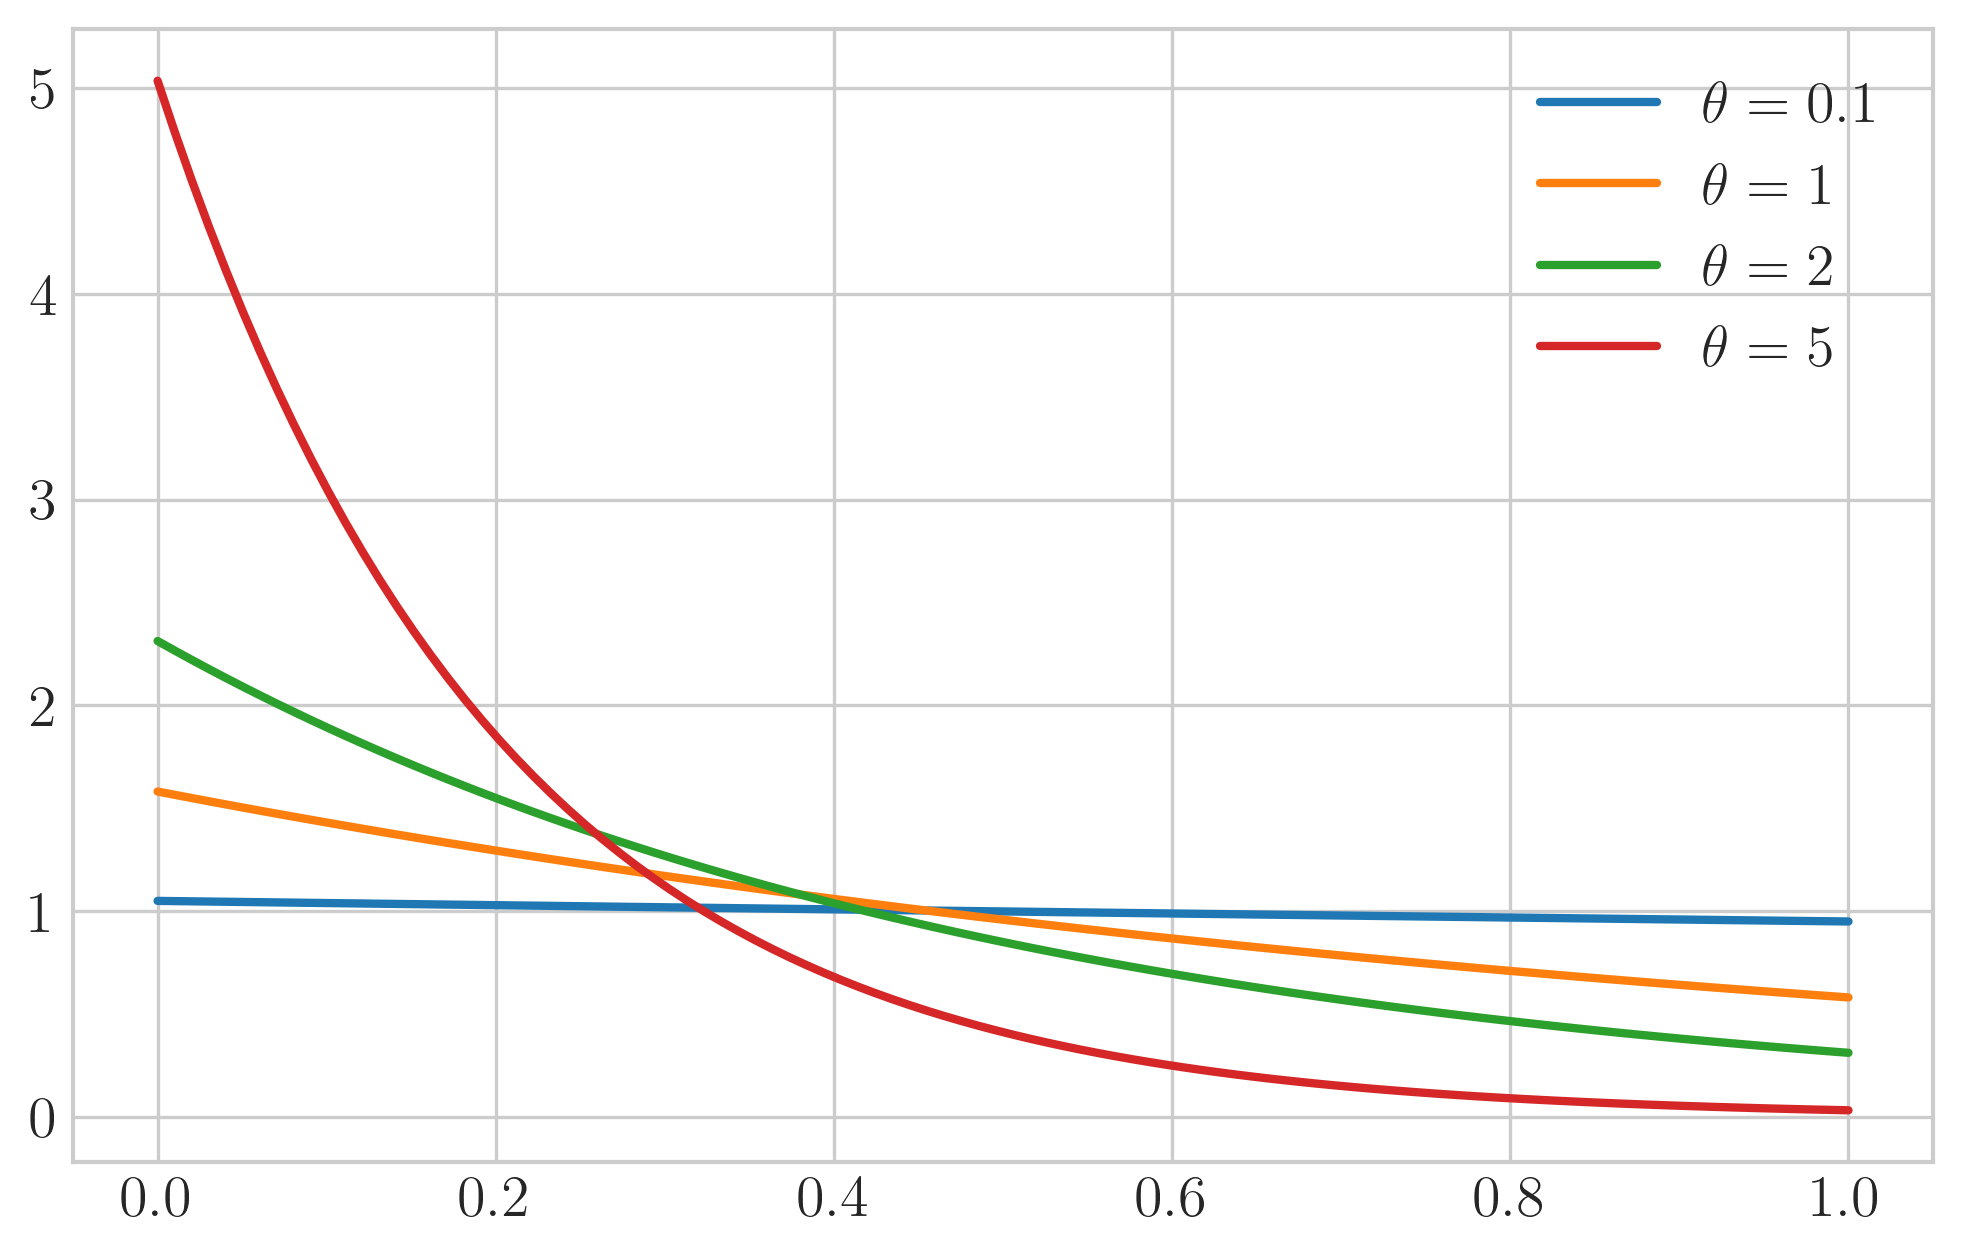
\includegraphics[scale=0.65]{plots/pdf_min_hat.png}
        \caption{Графіки щільності $f_{\widehat{m}}(x)$ для різних значень $\theta$.}
    \end{figure}
    \begin{figure}[H]
        \centering
        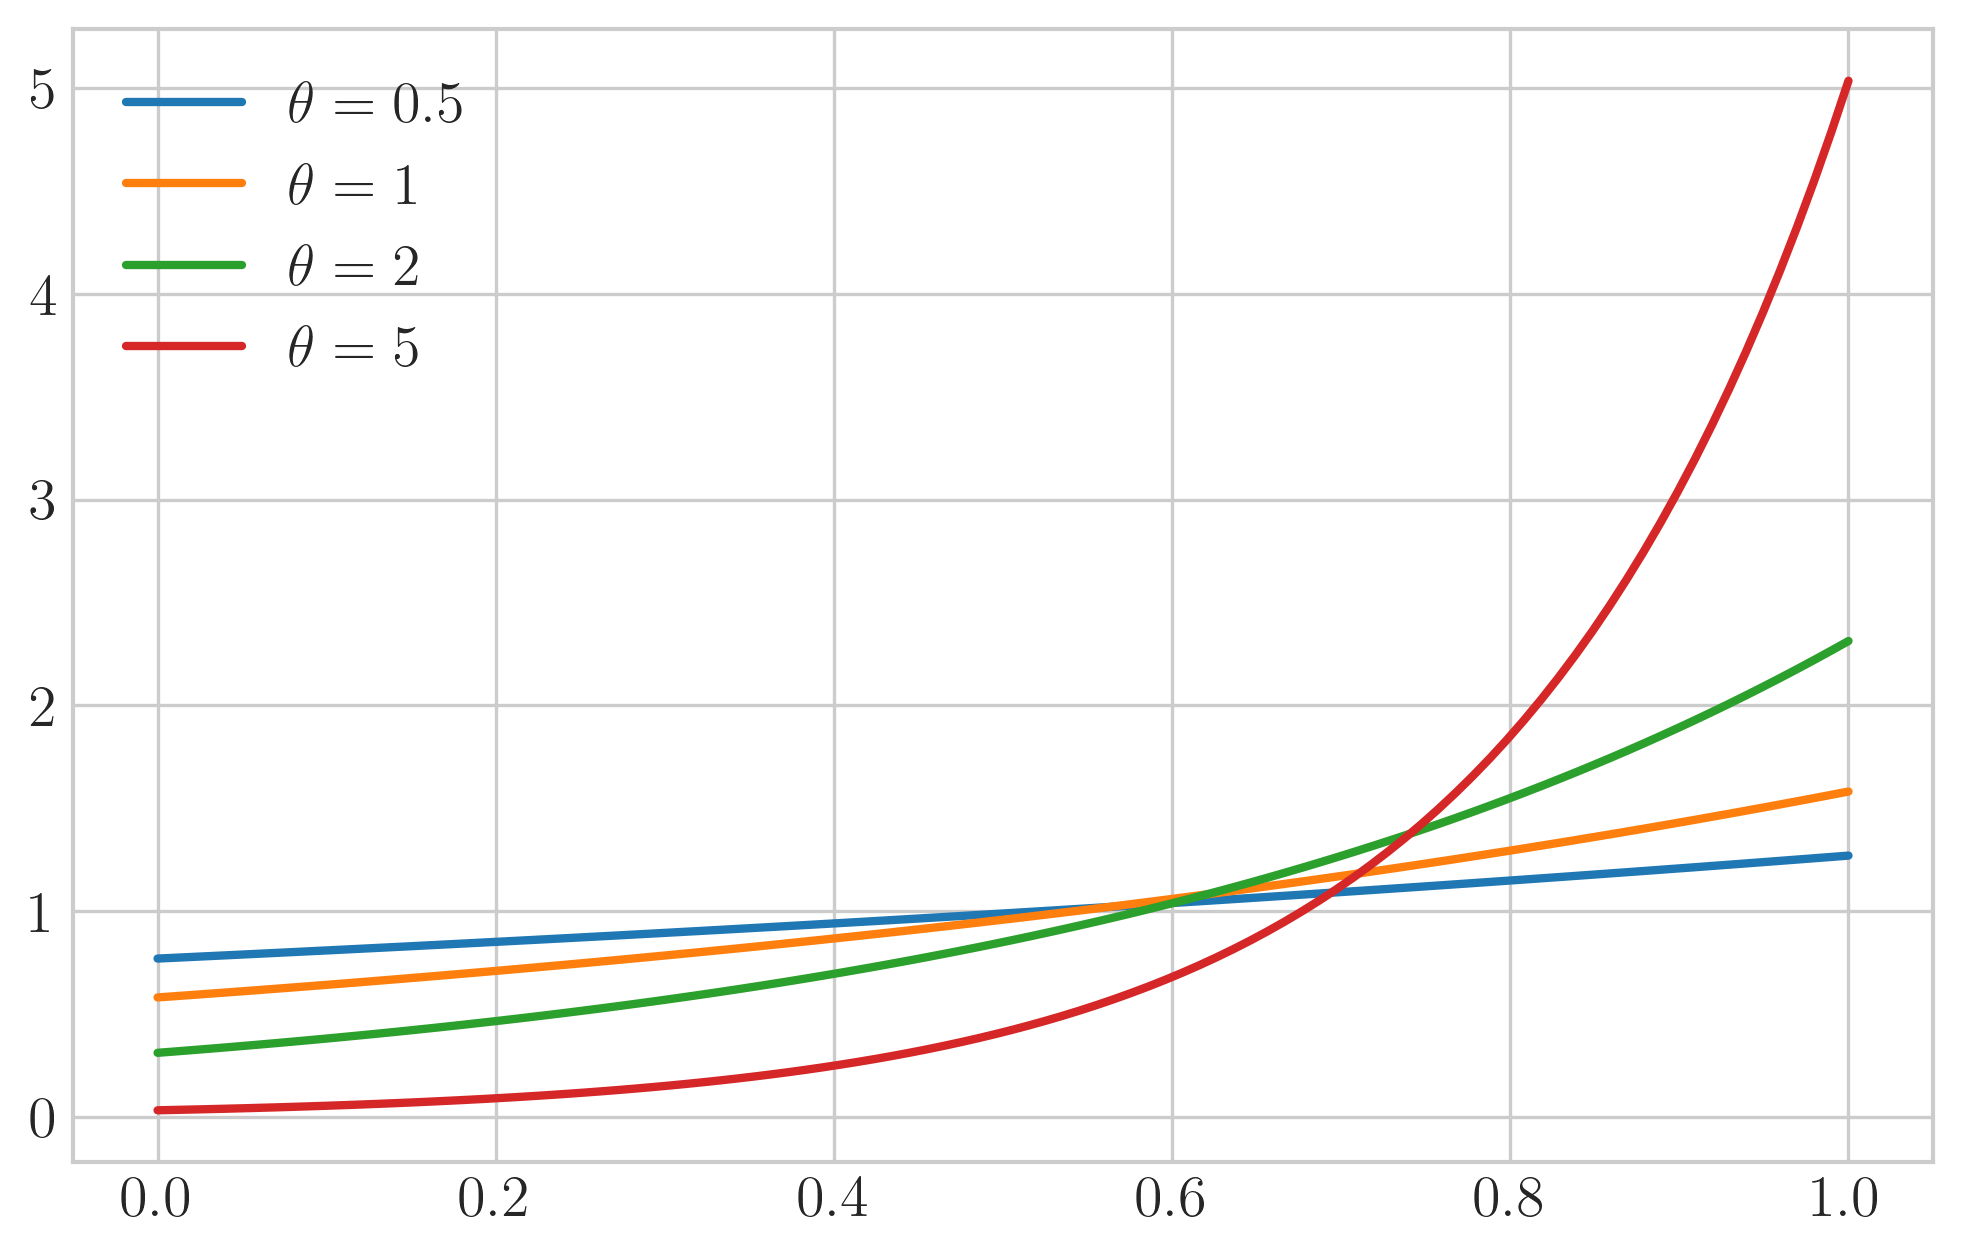
\includegraphics[scale=0.65]{plots/pdf_max_hat.png}
        \caption{Графіки щільності $f_{\widehat{M}}(x)$ для різних значень $\theta$.}
    \end{figure}
\end{theorem}

\subsection{Сума нерухомих точок}
Граничний розподіл суми нерухомих точок можна отримати, користуючись функціоналом Лапласа точкового процесу Пуассона.
Згідно з означенням \ref{def:poiss_proc}, для процесу Пуассона з мірою інтенсивності 
$\theta \cdot \mathrm{Leb}$ на $[0, 1]$ цей функціонал задається як
\begin{equation}\label{laplace_functional}
    \psi_N(f) = \exp\left\{ - \; \theta \int_0^1 \left(1 - e^{-f(x)}\right) \d x\right\}
\end{equation}
для вимірних, невід'ємних, обмежених функцій $f$ на $[0, 1]$.

Позначатимемо $\Sum(N)$ суму атомів точкового процесу Пуассона $N$. 
Для будь-якої точкової міри $\mu$, 
$\Sum(\mu) = \int_0^1 x \d\mu$. 
Перетворення Лапласа невід'ємної випадкової величини $X$ задається
$\L{X}(p) = \E e^{-pX}$. 
Якщо порівняти це означення з \eqref{laplace_functional}, можна побачити, що
перетворення Лапласа $\Sum(N)$ дорівнює значенню $\psi_N(f)$ для $f(x) = px$.
Пряме обчислення дає наступний результат:
\begin{gather}\label{laplace_of_sum}
    \L{\Sum(N)}(p) = 
    \exp\left\{- \theta \left( 1 + \frac{1}{p}(e^{-p} - 1)\right) \right\}.
\end{gather}

Оскільки розподіл $\Sum(N)$ є сумішшю абсолютно неперервного розподілу та
дискретного з атомом в 0, можна знайти перетворення Лапласа
лише абсолютно неперервної частини, що також буде перетворення для
$\Sum(\widehat{N})$.
\begin{gather}
    \L{\Sum(N)}(p) = \E e^{-p\cdot\Sum(N)} = 
    1 \cdot \P{\Sum(N) = 0} + \nonumber \\ +
    \E e^{-p\cdot\Sum(\widehat{N})} \cdot \P{\Sum(N) > 0} =
    e^{-\theta} + \L{\Sum(\widehat{N})}(p) \cdot (1-e^{-\theta})
    \nonumber \\
    \L{\Sum(\widehat{N})}(p) = \frac{1}{1 - e^{-\theta}}
    \left(\L{\Sum(N)}(p) - e^{-\theta}\right) = \nonumber \\ =
    \label{laplace_of_sum_cont}
    \frac{e^{-\theta}}{1 - e^{-\theta}} \cdot 
    \left(\exp\left\{- \frac{\theta}{p}(e^{-p} - 1) \right\} - 1\right)
\end{gather}

$\Sum(\widehat{N})$ є абсолютно неперервною випадковою величиною,
$\L{\Sum(\widehat{N})}(p)$ є перетворенням Лапласа для щільності, тому
перетворення Лапласа для функції розподілу $\Sum(\widehat{N})$
задається 
\begin{equation}\label{sum_cdf_laplace}
    \L{F_{\Sum(\widehat{N})}(x)}(p) = 
    \frac{e^{-\theta}}{1 - e^{-\theta}} \cdot \frac{1}{p} \cdot
    \left(\exp\left\{- \frac{\theta}{p}(e^{-p} - 1) \right\} - 1\right)
\end{equation}
Знаходження оберненого перетворення для \eqref{sum_cdf_laplace}
є доволі складним.

Розглянемо інший підхід до знаходження $F_{\Sum(N)}(x) = \P{\Sum(N) \leq x}$:
\begin{gather*}
    \P{\Sum(N) \leq x} = 
    \sum_{m=0}^{\infty} \P{\Sum(N) \leq x \mid N([0, 1]) = m} \P{N([0, 1]) = m}
    = \\ = \mathds{1}\left\{x\geq 0\right\}\cdot e^{-\theta} +
    \sum_{m=1}^{\infty} \P{\Sum(N) \leq x \mid N([0, 1]) = m} \frac{\theta^m}{m!} e^{-\theta}
\end{gather*}
Згідно з \cite{ContUnivDistr} (ст. 296), умовні розподіли 
$\P{\Sum(N) \leq x \mid N([0, 1]) = m}$
є розподілами Ірвіна-Голла --- розподілами 
суми $m$ незалежних випадкових величин з розподілом $\Unif{0, 1}$. Їх
функція розподілу має вигляд
\begin{gather*}
    F_s^{[m]} (x) = \begin{cases}
        0, & x < 0, \\
        \frac{1}{m!}\sum_{k=0}^{\floor*{x}} (-1)^k C_m^k (x-k)^m, & 0 \leq x < m, \\
        1, & x \geq m.
    \end{cases}
\end{gather*}
Для кожного інтервалу $[n, n+1)$, $n\in \N_0$, 
$\P{\Sum(N) \leq x}$  може бути виражена через $I_{\nu}(z)$, $\nu \in \R$  ---
модифіковані функції Бесселя першого роду (\cite{Abramowitz_Stegun}, ст. 375):
\begin{equation*}
    I_{\nu}(z) = \left(\frac{1}{2} z\right)^{\nu}
    \sum_{k=0}^{\infty} \frac{
        \left(\frac{1}{4} z^2 \right)^{k}
    }{
        k! \Gamma(\nu + k + 1)
    }
\end{equation*}
Отримаємо відповідну формулу. Нехай $x \in [n, n+1)$,
\begin{gather*}
    e^{\theta} \cdot \P{\Sum(N) \leq x} = 
    1 + \sum_{m=1}^{\infty} \P{\Sum(N) \leq x \mid N([0, 1]) = m} \frac{\theta^m}{m!} = \\ =
    1 + \sum_{m=1}^{n} 1 \cdot \frac{\theta^m}{m!} + 
    \sum_{m=n+1}^{\infty} \left(
        \frac{1}{m!}\sum_{k=0}^{n} (-1)^k C_m^k (x-k)^m
    \right) \frac{\theta^m}{m!} = \\ =
    \sum_{m=0}^{n} \frac{\theta^m}{m!} + 
    \sum_{m=n+1}^{\infty} \left(
        \sum_{k=0}^{n} (-1)^k \frac{1}{k! (m-k)!} (x-k)^m
    \right) \frac{\theta^m}{m!} = \\ =
    \sum_{m=0}^{n} \frac{\theta^m}{m!} + 
    \sum_{k=0}^{n} \frac{(-1)^k}{k!} \left(
        \sum_{m=n+1}^{\infty} \frac{1}{m! (m-k)!} (x - k)^m \theta^m
    \right) = \left[m - k = l \right] = \\
    = \sum_{m=0}^{n} \frac{\theta^m}{m!} + 
    \sum_{k=0}^{n} \frac{(-1)^k}{k!} \left(
        \sum_{l=n-k+1}^{\infty} \frac{1}{l! (l+k)!} (x - k)^{l+k} \theta^{l+k}
    \right) = \\ =
    \sum_{m=0}^{n} \frac{\theta^m}{m!} + 
    \sum_{k=0}^{n} \frac{(-1)^k}{k!} (x-k)^k \theta^k
    \left(
        \sum_{l=n-k+1}^{\infty} \frac{1}{l! (l+k)!} (x - k)^{l} \theta^{l}
    \right) = \\ = \left[\frac{1}{l! (l+k)!} (x - k)^{l} \theta^{l} = a_{k, l}\right] = \\ =
    \sum_{m=0}^{n} \frac{\theta^m}{m!} +
    \sum_{k=0}^{n} \frac{(-1)^k}{k!} (x-k)^k \theta^k
    \left(
        \sum_{l=0}^{\infty} a_{k, l} - 
        \sum_{l=0}^{n-k} a_{k, l} 
    \right) = \\
    = \sum_{k=0}^{n} \frac{(-1)^k}{k!}
    \left(\theta (x - k)\right)^{\frac{k}{2}} I_k\left(2\sqrt{\theta(x-k)}\right) + \\ +
    \sum_{m=0}^{n} \frac{\theta^m}{m!}
    - \sum_{k=0}^{n} \sum_{l=0}^{n-k}  \frac{(-1)^k}{k!} \frac{1}{l! (l+k)!} (x - k)^{k+l} \theta^{k+l}
\end{gather*} 
Позначимо $R(n) = \sum_{m=0}^{n} \frac{\theta^m}{m!}$,
$L(n) = \sum_{k=0}^{n} \sum_{l=0}^{n-k} \frac{(-1)^k}{k!} \frac{1}{l! (l+k)!} (x - k)^{k+l} \theta^{k+l}$.
Покажемо, що $R(n) - R(n-1) = L(n) - L(n-1)$ для всіх $n \in \N$:
\begin{gather*}
    R(n) - R(n-1) = \frac{\theta^n}{n!}, \\
    L(n) - L(n-1) = \sum_{k=0}^n \sum_{l=0}^{n-k} s_{k, l} - 
    \sum_{k=0}^{n-1} \sum_{l=0}^{n-k-1} s_{k, l} = \sum_{i=0}^n s_{i, n-i} = \\ =
    \sum_{i=0}^n \frac{(-1)^i}{i!} \frac{1}{(n-i)! n!} (x - i)^n \theta^n = 
    \frac{\theta^n}{n!} \cdot \frac{1}{n!} \sum_{i=0}^n (-1)^i C_n^i (x-i)^n.
\end{gather*}
Розглянемо функцію $f(x) = x^n$.
Ліва скінченна різниця першого порядку для $f$ з кроком $h=1$ --- це 
$\Delta f(x) = f(x) - f(x-1)$, другого порядку --- $\Delta^2 f(x) = \Delta f(x) - \Delta f(x-1) = 
f(x) - 2f(x-1) + f(x-2)$,
аналогічно рекурентно визначаються скінченні різниці вищих порядків.
Загальною формулою для різниці $k$-того порядку буде
$\Delta^k f(x) = \sum_{i=0}^k (-1)^i C_k^i f(x-i) = \sum_{i=0}^k (-1)^i C_k^i (x - i)^n$,
тому вираз $\sum_{i=0}^n (-1)^i C_n^i (x-i)^n$ --- це ліва скінченна різниця $n$-того порядку для
$x^n$. Оскільки кожна скінченна різниця є поліном порядку на 1 менше, ніж попередня,
то різниця $n$-того порядку вже буде константою. Виявляється,
що
\begin{gather*}
    \frac{1}{n!} \Delta^n f(n) = 
    \frac{1}{n!} \sum_{i=0}^n (-1)^i C_n^i (n - i)^n = 
    \frac{1}{n!} \sum_{k=0}^n (-1)^{n-k} C_n^k k^n = {n\brace n} = 1,
\end{gather*}
де ${n \brace m}$ позначає число Стірлінґа другого роду (\cite{Abramowitz_Stegun}, ст. 824-825).
Отже, $R(n) - R(n-1) = L(n) - L(n-1)$ для всіх $n \in \N$. Оскільки
$R(0) = L(0) = 1$, то $R(n) = L(n)$ для всіх $n \in \N$.
Таким чином, отримуємо 
\begin{gather}
    F_{\Sum(N)}(x) = e^{-\theta}
    \sum_{k=0}^{n} \frac{(-1)^k}{k!}
    \left(\theta (x - k)\right)^{\frac{k}{2}} I_k\left(2\sqrt{\theta(x-k)}\right), \; x \in [n, n+1)
\end{gather}

В свою чергу, функція розподілу $\Sum(\widehat{N})$ 
може бути виражена через $F_{\Sum(N)}(x)$ наступним чином:
\begin{gather}
    \P{\Sum(\widehat{N}) \leq x} = \P{\Sum(N) \leq x \mid \Sum(N) > 0} = 
    \begin{cases}
        0, & x < 0, \\
        \frac{F_{\Sum(N)}(x) - e^{-\theta}}{1-e^{-\theta}}, & x \geq 0.
    \end{cases}
\end{gather}

При цьому, $\E\Sum(N)$ значно простіше знайти
за формулою повного математичного сподівання,
оскільки для $m > 0$ $\E\left(\Sum(N) \mid N([0, 1]) = m\right) = \frac{m}{2}$
як математичне сподівання суми $m$ незалежних випадкових величин
з розподілом $\Unif{0, 1}$:
\begin{gather*}
    \E\Sum(N) = 0\cdot \P{N([0, 1]) = 0} +
    \sum_{m=1}^{\infty} \frac{m}{2} \frac{\theta^m}{m!} e^{-\theta} =
    \frac{e^{-\theta}}{2}\sum_{m=1}^{\infty} \frac{\theta^m}{(m-1)!} = \frac{\theta}{2}
\end{gather*}

Сформулюємо отриманий результат у вигляді теореми.
\begin{theorem}
    Нехай $\sigma \sim \ESF{n, \theta}$, а 
    $S_n = \sum_{i : \sigma(i) = i} i = \sum_{i=1}^n i \cdot \mathds{1}\left\{\sigma(i) = i \right\}$ --- сума нерухомих точок $\sigma$.
    Тоді при $n\to\infty$ виконується граничне
    співвідношення
    $\frac{S_n}{n} \overset{d}{\longrightarrow} S$,
    де функція розподілу випадкової величини $S$ дорівнює
    \begin{gather}
        F_{S}(x) = \begin{cases}
            0, & x < 0, \\
            e^{-\theta}
            \sum\limits_{k=0}^{\floor*{x}}
            (-1)^k \frac{1}{k!}\left(\theta(x-k)\right)^{\frac{k}{2}} I_k\left(2\sqrt{\theta(x-k)}\right), & x \geq 0,
        \end{cases}
    \end{gather}
    а її перетворення Лапласа має вигляд \eqref{laplace_of_sum}.
    
    Якщо позначити $\widehat{S}_n$ суму нерухомих точок за умови,
    що вони взагалі існують, то виконуються також граничне співвідношення
    $\frac{\widehat{S}_n}{n} \overset{d}{\longrightarrow} \widehat{S}$,
    де функція розподілу випадкової величини $S$ дорівнює
    \begin{gather}
        F_{\widehat{S}}(x) = \begin{cases}
            0, & x < 0, \\
            \frac{F_{S}(x) - e^{-\theta}}{1 - e^{-\theta}}, & x \geq 0,
        \end{cases},
    \end{gather}
    а її перетворення Лапласа має вигляд \eqref{laplace_of_sum_cont}.
    \begin{figure}[H]
        \centering
        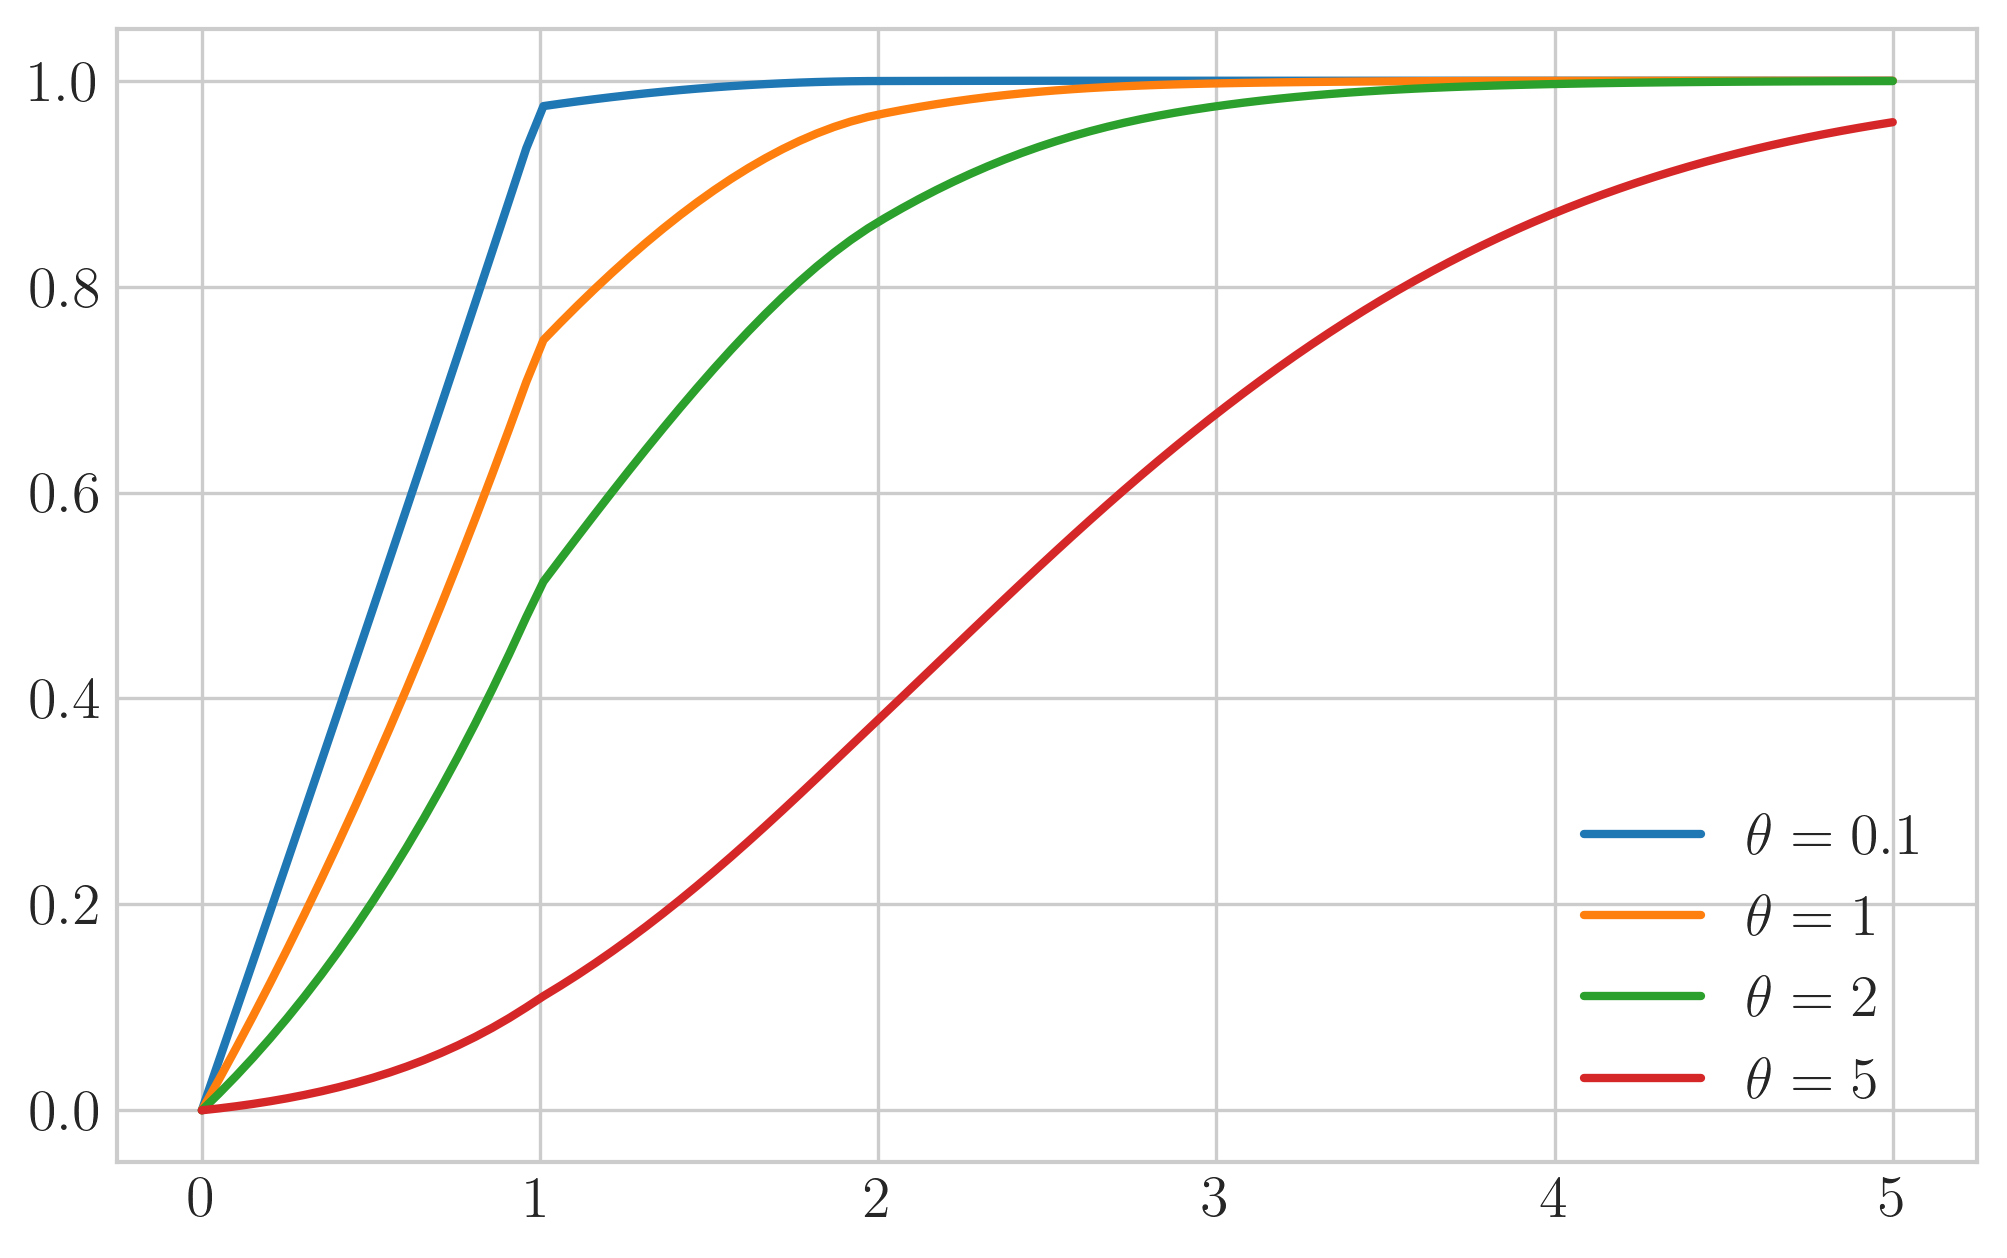
\includegraphics[scale=0.65]{plots/cdf_sum_hat.png}
        \caption{Графіки функції розподілу $F_{\widehat{S}}(x)$ для різних значень $\theta$.}
    \end{figure}
\end{theorem}

\subsection{Найменші і найбільші спейсинги}
Визначимо граничні розподіли найменшого і найбільшого спейсингів --- відстаней
між нерухомими точками.
\begin{remark}
    Щоб застосувати тут теоретичні результати, що стосуються
    випадкового розбиття інтервалів, зручно вважати
    $\min(N)$ і $1-\max(N)$ спейсингами. Для випадкової
    перестановки $\left\{1, \dots, n\right\}$ це означатиме
    вважати $0$ та $n+1$ <<штучними>> нерухомими точками.
\end{remark}

Нехай $U_1, U_2, \dots, U_{n}$ ---
незалежні випадкові величини
з розподілом $\Unif{0, 1}$, що розділяють відрізок $[0, 1]$ на $n+1$
інтервалів з довжинами $S_1, S_2, \dots, S_{n+1}$, або, у відсортованому вигляді, 
$S_{(1)}^{[n+1]} < S_{(2)}^{[n+1]} < \dots < S_{(n+1)}^{[n+1]}$
(нагадаємо, $S_{(i)}$ позначає $i$-ту порядкову статистику, а
$S_{(i)}^{[n+1]}$ --- те ж саме, але з вказанням $n+1$ як кількості цих статистик).
Розподіли $S_{(k)}^{[n+1]}$ отримано у багатьох роботах
(наприклад, \cite{Holst_1980}, \cite{Pinelis_2019}). Зокрема, для $x\in[0,1]$
\begin{gather}
    \label{min_spacing}
    \P{S_{(1)}^{[n+1]} > x} = \left((1-(n+1)x)_+\right)^n, \\
    \label{max_spacing}
    \P{S_{(n+1)}^{[n+1]} > x} = 
    \sum_{j=1}^{n+1} (-1)^{j-1} C_{n+1}^j \left((1-jx)_+\right)^n,
\end{gather}
де $x_+ = \max(x, 0)$.

Отже, розподіли найменшого $\smin(N)$ та найбільшого $\smax(N)$ спейсингів 
між атомами $N$ задаються
(з домовленістю $S_{(1)}^{1} = 1$)
\begin{gather}
    \label{s_min}
    \P{\smin(N) > x} = 
    \sum_{n=0}^{\infty} \P{S_{(1)}^{[n+1]} > x} \P{N([0, 1]) = n} \\
    \label{s_max}
    \P{\smax(N) > x} = 
    \sum_{n=0}^{\infty} \P{S_{(n+1)}^{[n+1]} > x} \P{N([0, 1]) = n}
\end{gather}
Хоча явні вирази для \eqref{s_min} та \eqref{s_max},
скоріш за все, доволі складні, цікаво звернути увагу на дві випадкові величини
з такими ж розподілами.

Відомо (наприклад, \cite{Holst_1980}), що для незалежних величин 
$X_1, X_2, \dots, X_{n+1}$ з розподілом $\Exp{1}$
мають місце наступні три рівності:
\begin{gather}
    \label{distr_equal_1}
    \left(
        S_1, S_2, \dots, S_{n+1}
    \right)^T
    \overset{d}{=}
    \left(
        \frac{X_1}{\sum_{i=1}^{n+1} X_i},
        \frac{X_2}{\sum_{i=1}^{n+1} X_i},
        \dots,
        \frac{X_{n+1}}{\sum_{i=1}^{n+1} X_i}
    \right)^T \\
    \label{distr_equal_2}
    \left(
        S_{(1)}, S_{(1)}, \dots, S_{(n+1)}
    \right)^T
    \overset{d}{=}
    \left(
        \frac{X_{(1)}}{\sum_{i=1}^{n+1} X_i},
        \frac{X_{(2)}}{\sum_{i=1}^{n+1} X_i},
        \dots,
        \frac{X_{(n+1)}}{\sum_{i=1}^{n+1} X_i}
    \right)^T \\
    \label{distr_equal_3}
    X_{(i)} \overset{d}{=}
    \frac{X_{n+1}}{n+1} + \frac{X_{n}}{n} + \dots + \frac{X_{n-i+2}}{n-i+2} = 
    \sum_{k=0}^{i-1} \frac{X_{n+1-k}}{n+1-k}
\end{gather}
Рівності \eqref{distr_equal_2} та \eqref{distr_equal_3}
можна узагальнити в наступну рівність:
\begin{lemma}\label{distr_equal}
    Для порядкових статистик спейсингів 
    $S_{(1)}^{[n+1]}, ..., S_{(n+1)}^{[n+1]}$
    між незалежними величинами з розподілом $\Unif{0, 1}$
    та незалежних величин 
    $X_1, X_2, \dots, X_{n+1}$ з розподілом $\Exp{1}$ має місце
    рівність 
    \begin{gather}\label{distr_equal_4}
        S_{(i)}^{[n+1]} \overset{d}{=}
        \frac{
            \frac{X_{n+1}}{n+1} + \frac{X_{n}}{n} + \dots + \frac{X_{n-i+2}}{n-i+2}
        }{
            \sum_{j=1}^{n+1} X_j
        } = \frac{
            \sum_{k=0}^{i-1} \frac{X_{n+1-k}}{n+1-k}
        }{
            \sum_{j=1}^{n+1} X_j
        }, \; i = 1, \dots, n
    \end{gather}
\end{lemma}
\begin{proof}
    Позначимо спейсинги між $X_1, X_2, \dots, X_{n+1}$ через
    $\Delta_1 = X_{(1)}$,
    $\Delta_i = X_{(i)} - X_{(i-1)}, i=2, \dots, n+1$. З \cite{Arnold_et_al_2008} відомо, що
    всі $\Delta_i$ незалежні та мають розподіли $\Exp{n-i+2}$.
    Отже, праву частину $S_{(i)} \overset{d}{=} \frac{X_{(i)}}{\sum_{j=1}^{n+1}X_j}$
    можна переписати як
    \begin{gather*}
        \frac{X_{(i)}}{\sum_{j=1}^{n}X_j} = 
        \frac{X_{(i)}}{\sum_{j=1}^{n}X_{(j)}} = 
        \frac{
            \Delta_1 + \dots + \Delta_i
        }{
            \Delta_1 + \left(\Delta_1 + \Delta_2\right) +
            \dots + \left(\Delta_1 + \dots + \Delta_n\right)
        }
    \end{gather*}
    Введемо нові незалежні випадкові величини
    $Y_i = (n-i+2)\Delta_i$ з розподілом
    $\Exp{1}$. В термінах $Y_i$,
    верхню рівність можна переписати як
    \begin{gather*}
        \frac{X_{(i)}}{\sum_{j=1}^{n+1}X_j} = 
        \frac{
            \sum_{j=1}^i \frac{Y_j}{n-j+2} 
        }{
            \sum_{j=1}^{n+1} Y_j
        }
    \end{gather*}
    Оскільки $X_i$ та $Y_i$ незалежні та мають однакові розподіли, то отримуємо \eqref{distr_equal_4}.
\end{proof}

Окремими випадками леми \ref{distr_equal}
є рівності для мінімального і максимального спейсингів
$S_{(1)}^{[n+1]} \overset{d}{=} \frac{X_{n+1}}{(n+1)\sum_{i=1}^{n+1} X_i}$
та $S_{(n+1)}^{[n+1]} \overset{d}{=} \frac{\sum_{i=1}^{n+1} \frac{X_i}{n-i+2}}{\sum_{i=1}^{n+1} X_i}
\overset{d}{=} \frac{\sum_{i=1}^{n+1} \frac{X_i}{i}}{\sum_{i=1}^{n+1} X_i}$.
Разом з \eqref{s_min} та \eqref{s_max}
вони приводять до наступних рівностей за розподілом:
\begin{gather}\label{distr_equal_5}
    \smin(N) \overset{d}{=}
    \frac{X_{\nu+1}}{(\nu+1)\sum_{i=1}^{\nu+1} X_i} , \;
    \smax(N) \overset{d}{=} 
    \frac{\sum_{i=1}^{\nu+1} \frac{X_i}{i}}{\sum_{i=1}^{\nu+1} X_i}
\end{gather}
де $\nu$ має розподіл $\Poiss{\theta}$, а $\left(X_i, i\geq 1\right)$ незалежні і мають розподіл $\Exp{1}$.

Відповідні математичні сподівання $\E\smin(N)$ та $\E\smax(N)$ можна знайти з \eqref{distr_equal_5}. 
Нехай $n \in \N_0$, тоді
\begin{gather*}
    \E\left(
        \frac{X_{n+1}}{(n+1)\sum_{i=1}^{n+1} X_i}
    \right) = \frac{1}{(n+1)^2}\cdot \E \left(
        \frac{X_1}{\sum_{i=1}^{n+1} X_i} + \dots + \frac{X_{n+1}}{\sum_{i=1}^{n+1} X_i}
    \right) = \frac{1}{(n+1)^2} \\
    \E\left(
        \frac{\sum_{i=1}^{n+1} \frac{X_i}{i}}{\sum_{i=1}^{n+1} X_i}
    \right) = 
    \sum_{i=1}^{n+1} \frac{1}{i} \cdot \E\left(\frac{X_i}{\sum_{i=1}^{n+1} X_i}\right) = 
    \frac{1}{n+1} \cdot \sum_{i=1}^{n+1} \frac{1}{i}
\end{gather*}
Оскільки $\P{\nu = n} = \frac{\theta^n}{n!}e^{-\theta}$, то
\begin{gather*}
    \E\smin(N) = \frac{e^{-\theta}}{\theta}\sum_{n=1}^{\infty} \frac{\theta^n}{n\cdot n!} = 
    \frac{e^{-\theta}}{\theta}\int_0^\theta \frac{e^t-1}{t}\d t, \\
    \E\smax(N) = \frac{e^{-\theta}}{\theta}\sum_{n=1}^{\infty} \frac{H_n}{n!} \theta^n = 
    \frac{1}{\theta} \int_0^{\theta} \frac{1-e^{-t}}{t}\d t.
\end{gather*}
де $H_n = \sum_{k=1}^n \frac{1}{k}$ --- $n$-те гармонічне число.
Зокрема, для $\theta = 1$ (випадок рівномірного розподілу) 
$\E\smin(N) \approx 0.48483$ і $\E\smax(N) \approx 0.7966$.

Сформулюємо отриманий результат у вигляді теореми.
\begin{theorem}
    Нехай $\sigma \sim \ESF{n, \theta}$, а $\delta_n$ та $\Delta_n$ ---
    відповідно, найменша та найбільша відстані між нерухомими точками $\sigma$,
    де за домовленістю $0$ та $n+1$ вважаються нерухомими точками, тобто
    за відсутності нерухомих точок найбільша та найменша відстані обидві дорівнюють $n$.
    Тоді при $n\to\infty$ виконуються граничні
    співвідношення
    $\frac{\delta_n}{n} \overset{d}{\longrightarrow} \delta$ і 
    $\frac{\Delta_n}{n} \overset{d}{\longrightarrow} \Delta$, де
    \begin{gather}
        \delta \overset{d}{=}
        \frac{X_1}{(\nu+1)\sum_{i=1}^{\nu+1} X_i}, \;
        \Delta \overset{d}{=} 
        \frac{\sum_{i=1}^{\nu+1} \frac{X_i}{i}}{\sum_{i=1}^{\nu+1} X_i},
    \end{gather}
    для незалежних між собою $\left(X_i, i \geq 1\right)$
    з розподілом $\Exp{1}$ та $\nu \sim \Poiss{\theta}$,
    незалежної від $\left(X_i, i \geq 1\right)$.
\end{theorem}